\documentclass{article}

\title{Optics Notes}
\author{Henry Oehlrich}

\usepackage{tikz}
\usepackage{amsmath}
\usepackage[labelfont=bf]{caption}
\usepackage[margin=1.25in]{geometry}

\usetikzlibrary{arrows.meta}

\begin{document}
\maketitle

\section{Reflection}

\begin{figure}[ht]
    \begin{minipage}[b]{0.5\linewidth}
        \centering
        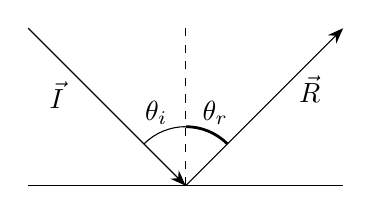
\begin{tikzpicture}
            \draw (-2,0) -- (2,0);
            \draw[dashed] (0,0) -- (0,2);

            \draw[-{Stealth[length=2mm]}] (-2,2) -- (0,0);
            \path (0,0) ++(145:2) node {$\vec{I}$};
            \draw[-{Stealth[length=2mm]}] (0,0) -- (2,2);
            \path (0,0) ++(38:2) node {$\vec{R}$};

            \draw (0,0.75) arc [start angle=90, end angle=135, radius=0.75];
            \path (0,0) ++(120:0.75) node[above] {$\theta_i$};
            \draw[line width=1pt] (0,0.75) arc [start angle=90, end angle=45, radius=0.75];
            \path (0,0) ++(60:0.75) node[above] {$\theta_r$};
        \end{tikzpicture}
        \caption{Specular Reflection}
        \label{fig:specular}
    \end{minipage}%
    \begin{minipage}[b]{0.5\linewidth}
        \centering
        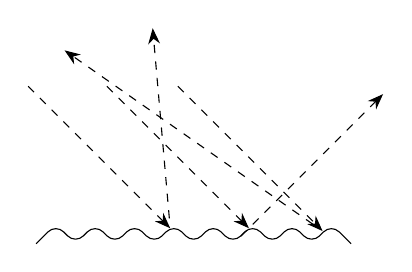
\begin{tikzpicture}
            \draw[rounded corners] (-1,0) -- ++(0.25,0.25) -- ++(0.25,-0.25) -- ++(0.25,0.25) -- ++(0.25,-0.25) --
                            ++(0.25,0.25) -- ++(0.25,-0.25) -- ++(0.25,0.25) -- ++(0.25,-0.25) --
                            ++(0.25,0.25) -- ++(0.25,-0.25) -- ++(0.25,0.25) -- ++(0.25,-0.25) --
                            ++(0.25,0.25) -- ++(0.25,-0.25) -- ++(0.25,0.25) -- ++(0.25,-0.25);

            \draw[dashed,-{Stealth[length=2mm]}] (-1.1,2) -- ++(-45:2.55) node(p1) {};
            \draw[dashed,-{Stealth[length=2mm]}] (p1) -- ++(95:2.55);
            \draw[dashed,-{Stealth[length=2mm]}] (-0.1,2) -- ++(-45:2.55) node(p2) {};
            \draw[dashed,-{Stealth[length=2mm]}] (p2) ++(-0.1,-0.1) -- ++(45:2.55);
            \draw[dashed,-{Stealth[length=2mm]}] (0.8,2) -- ++(-45:2.6) node(p3) {};
            \draw[dashed,-{Stealth[length=2mm]}] (p3) -- ++(145:4);

        \end{tikzpicture}
        \caption{Diffuse Reflection}
        \label{fig:diffuse}
    \end{minipage}
\end{figure}

\subsection{Mirrors}

\begin{figure}[ht]
    \centering
    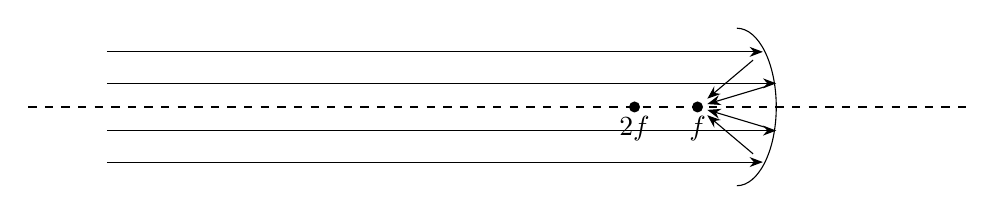
\begin{tikzpicture}
        \draw[dashed] (-6,0) -- (6,0);
        \draw (3,1) arc [start angle=90, end angle=-90, x radius=0.5, y radius=1];
        \fill (2.5,0) node[below] {$f$} node(f) {} circle [radius=0.07];
        \fill (1.7,0) node[below] {$2f$} node(2f) {} circle [radius=0.07];

        \draw[-{Stealth}] (-5,0.7) -- ++(8.33,0) node(p1) {};
        \draw[-{Stealth}] (p1) -- (f);
        \draw[-{Stealth}] (-5,0.3) -- ++(8.5,0) node(p2) {};
        \draw[-{Stealth}] (p2) -- (f);
        \draw[-{Stealth}] (-5,-0.3) -- ++(8.5,0) node(p3) {};
        \draw[-{Stealth}] (p3) -- (f);
        \draw[-{Stealth}] (-5,-0.7) -- ++(8.33,0) node(p4) {};
        \draw[-{Stealth}] (p4) -- (f);
    \end{tikzpicture}
    \caption{Parabolic Mirror}
    \label{fig:parabolic}
\end{figure}

\begin{figure}[ht]
    \begin{minipage}[b]{0.5\linewidth}
        \centering
        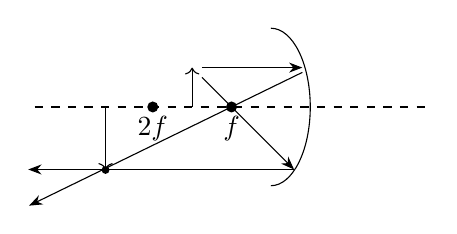
\begin{tikzpicture}
            \draw[dashed] (-3,0) -- (2,0);
            \draw (0,1) arc [start angle=90, end angle=-90, x radius=0.5, y radius=1];
            \fill (-0.5,0) node[below] {$f$} node(f) {} circle [radius=0.07];
            \fill (-1.5,0) node[below] {$2f$} node(2f) {} circle [radius=0.07];

            \draw[->] (-1,0) -- ++(0,0.5) node(p1) {};
            \draw[-{Stealth}] (p1) -- ++(1.4,0) node(p2)[right] {};
            \draw[-{Stealth}] (p2) -- ++(206:4);
            \draw[-{Stealth}] (p1) -- ++(-45:1.83) node(p3)[right] {};
            \draw[-{Stealth}] (p3) -- ++(-3.5,0);
            \fill (-2.1,-0.8) node(p4)[below] {} circle [radius=0.05];
            \draw[->] (-2.1,0) -- (p4);
        \end{tikzpicture}
        \caption{Convex Mirror}
        \label{fig:convex}
    \end{minipage}%
    \begin{minipage}[b]{0.5\linewidth}
        \centering
        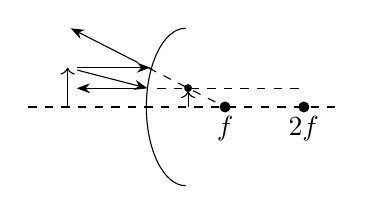
\begin{tikzpicture}
            \draw[dashed] (-2,0) -- (2,0);
            \draw (0,-1) arc [start angle=270, end angle=90, x radius=0.5, y radius=1];
            \fill (0.5,0) node[below] {$f$} node(f) {} circle [radius=0.07];
            \fill (1.5,0) node[below] {$2f$} node(2f) {} circle [radius=0.07];

            \draw[->] (-1.5,0) -- ++(0,0.5) node(p1) {};
            \draw[-{Stealth}] (p1) -- ++(1.05,0);
            \draw[dashed] (f) -- ++(153:1.1) node(p2) {};
            \draw[-{Stealth}] (p2) -- ++(153:1.1);
            \draw[-{Stealth}] (p1) -- ++(-14.5:1.05) node(p3) {};
            \draw[-{Stealth}] (p3) -- ++(-0.9,0);
            \draw[dashed] (p3) -- ++(2,0);
            \fill (0.03,0.24) circle [radius=0.05];
            \draw[->] (0.03,0) -- ++(0,0.2);
        \end{tikzpicture}
        \caption{Concave Mirror}
        \label{fig:concave}
    \end{minipage}%
\end{figure}

\newpage

\subsubsection{Mirror Equations}

\begin{figure}[ht]
    \centering
    \begin{tikzpicture}
        \draw[dashed] (-3,0) -- (3,0);
        \draw (0,1) arc [start angle=90, end angle=-90, x radius=0.5, y radius=1];
        \path (-1,0) node[above] {$+h$} node[below] {$-h$};
        \path (0.45,0.3) node[left] {$+d$} node[right] {$-d$};
    \end{tikzpicture}
    \caption{Mirror Sign Convention}
    \label{fig:mirror_sign}
\end{figure}

\begin{figure}[ht]
    \begin{minipage}[b]{0.5\linewidth}
        \begin{gather}
            \frac{1}{f} = \frac{1}{d_o} + \frac{1}{d_i} \\
            f = \frac{d_o*d_i}{d_o + d_i} \\
            d_o = \frac{d_i*f}{d_i - f} \\
            d_i = \frac{d_o*f}{d_o - f}
        \end{gather}
        \captionof{figure}{Mirror Equation}
        \label{fig:mirror_eq}
    \end{minipage}
    \begin{minipage}[b]{0.5\linewidth}
        \begin{gather}
            \frac{h_i}{h_o} = -\frac{d_i}{d_o} \\
            h_i = -\frac{d_i*h_o}{d_o} \\
            d_i = -\frac{h_i*d_o}{h_o}
        \end{gather}
        \captionof{figure}{Magnification Equation}
        \label{fig:mag_eq}
    \end{minipage}
\end{figure}

\section{Refraction}

\begin{figure}[ht]
    \begin{minipage}[b]{0.5\linewidth}
        \centering
        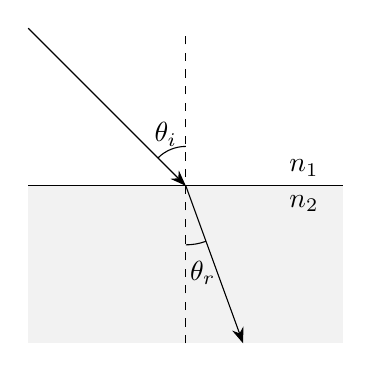
\begin{tikzpicture}
            \draw (-2,0) -- (2,0);
            \fill[ultra nearly transparent] (-2,0) rectangle (2,-2);
            \fill[transparent] (-2,0) rectangle (2,2);
            \draw[dashed] (0,-2) -- (0,2);
            \path (1.5,0) node[above] {$n_1$} node[below] {$n_2$};

            \draw[-{Stealth[length=2mm]}] (0,0) ++(135:2.83) -- (0,0);
            \draw (0,0.5) arc [start angle=90, end angle=135, radius=0.5] ++(0.1,0.3) node {$\theta_i$};
            \draw[-{Stealth[length=2mm]}] (0,0) -- (-70:2.13);
            \draw (0,-0.75) arc [start angle=-90, end angle=-70, radius=0.75] ++(-0.04,-0.4) node {$\theta_r$};
        \end{tikzpicture}
        \caption{Refraction where $n_1 < n_2$}
        \label{fig:refraction1}
    \end{minipage}%
    \begin{minipage}[b]{0.5\linewidth}
        \centering
        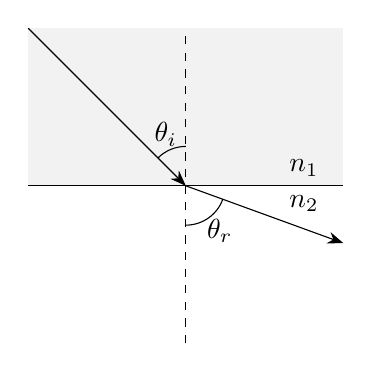
\begin{tikzpicture}
            \draw (-2,0) -- (2,0);
            \fill[transparent] (-2,0) rectangle (2,-2);
            \fill[ultra nearly transparent] (-2,0) rectangle (2,2);
            \draw[dashed] (0,-2) -- (0,2);
            \path (1.5,0) node[above] {$n_1$} node[below] {$n_2$};

            \draw[-{Stealth[length=2mm]}] (0,0) ++(135:2.83) -- (0,0);
            \draw (0,0.5) arc [start angle=90, end angle=135, radius=0.5] ++(0.1,0.3) node {$\theta_i$};
            \draw[-{Stealth[length=2mm]}] (0,0) -- (-20:2.13);
            \draw (0,-0.5) arc [start angle=-90, end angle=-20, radius=0.5] ++(-0.04,-0.4) node {$\theta_r$};
        \end{tikzpicture}
        \caption{Refraction where $n_1 > n_2$}
        \label{fig:refraction2}
    \end{minipage}
\end{figure}

\end{document}
